\section{Algoritmos de Análisis}
\label{sec:algAnalisis}
\torev{Última revisión: 20/06/12.}

Esta sección explicará con detalle los algoritmos de análisis de imágenes que se han desarrollado a lo largo del proceso de desarrollo. El objetivo de estos análisis es obtener, a partir de una imagen dada, información de los polígonos presentes tal y como se explica en la Sección~\ref{sec:representacionFiguras}. Esta información abarca tanto el color y vértices de cada polígono como qué polígonos se encuentran dentro de cuáles.\\

Puesto que nos interesa la eficiencia temporal del proceso de análisis para aumentar la comodidad de la experiencia de usuario, será necesario que los procesos de análisis no consuman mucho tiempo o, al menos, que permitan aumentar su velocidad mediante configuración externa. Es por ello que cada proceso de análisis contendrá parámetros mediante los cuales se podrá modificar la velocidad del análisis a costa de menor precisión en el mismo.\\

Para el diseño e implementación de los mismos se ha hecho uso de la librería multiplataforma de procesado de imágenes OpenCV {\cite{opencvDoc}). Esta librería, desarrollada por Intel y orientada a la visión por computador, ofrece multitud de funciones centradas principalmente en el procesado de imágenes en tiempo real.\\

Aunque en nuestros análisis no hagamos uso de sus funciones en tiempo real, sí que nos apoyaremos en sus subrutinas de procesado de imágenes para conseguir algoritmos que funcionen a velocidades deseadas. Estas subrutinas, que se detallarán más adelante, permiten detectar contornos y aproximarlos a polígonos, así como usar y operar imágenes de forma cómoda.\\

Para realizar el análisis ayudándondos de OpenCV, el proceso que se lleva a cabo consiste en:

\begin{itemize}

	\item \textbf{Detección de formas:} La imagen dada se transforma en una sucesión de imágenes binarias (únicamente en blanco y negro), donde las manchas blancas representan figuras independientes. Dado que varias figuras pueden superponerse (una figura contiene a otra), si se devolviera una única imagen binaria, sólo podría representarse una de las figuras (la que envuelve a las demás, ya que todas se pintaría como superficies blancas por ser figuras independientes), perdiendo información en el análisis. Es por ello que, siempre que resulte necesario, se devolverán varias imagenes de salida en esta fase del proceso, para asegurar que todas las figuras presentes se tienen en cuenta.\\
	
	En numerosas ocasiones se referirá a esta fase como ``filtrado de la imagen'' debido a que, para llevarse a cabo, se aplicarán filtros de procesado de imágenes sobre la imagen de entrada.
	
	\item\textbf{Detección de contornos y aproximación a polígonos:} Por cada mancha blancha, se recorre el perímetro en el mapa de bits y se almacena en una lista de puntos. Para finalizar, cada contorno se aproxima a un polígono y se analiza por separado, con el fin de desechar información no deseada y calcular datos relevantes. 
	
\end{itemize}

	Mientras que para la última fase existen rutinas de openCV que realizan casi toda la funcionalidad deseada, la primera fase requiere un estudio más exhaustivo.\\
	
	\subsection{Detección de formas}
	
	Para llevar a cabo esta primera fase se han probado y evaluado cinco métodos distintos. Se detallarán a continuación todos ellos.
	
	\subsubsection{Threshold}
	
	Consiste en aplicar un filtro de paso alta con respecto a un umbral de gris dado como entrada. Para ello, la imagen se convierte de 3 canales (rojo, verde y azul) a una de 1 único canal (escala de grises). Posteriormente se le aplica la siguiente transformación a cada píxel de la imagen:

	\begin{center}
		$pixel(x,y) = \left\{
		\begin{array}{cc}
		MAXVAL 	& \text{ cuando } pixel(x,y) > umbral\\ 
		0 	    & 	\text{e.o.c.}
		\end{array}\right.$
	\end{center}

	donde $MAXVAL$ representa el máximo valor que puede tener un pixel en un canal determinado (será 255 o 1, dependiendo de la representación de la imagen).\\
	
	Este filtro produce una única imagen de salida donde las zonas blancas conexas se interpretan como figuras independientes. Es por ello que, si dos manchas de color se comportan de igual manera ante el filtro (porque su color predominante es inferior o superior al umbral en ambas manchas), y se encuentran superpuestas una respecto de la otra, en la salida aparecerán como una única mancha blanca conexa, por lo que se considerará como una única figura (Figura~\ref{fig:threshold1}.)\\
	
		\begin{figure}[!htbp]
		\centering
		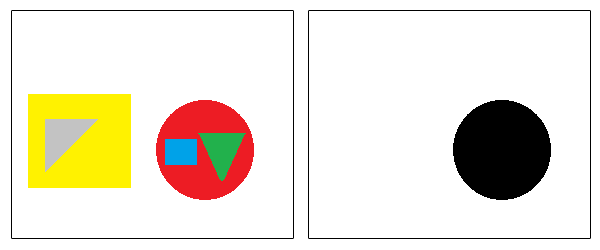
\includegraphics[scale=0.47]{graphics/threshold1.png}
		\caption{Ejemplo de filtrado threshold con umbral a 100}
		\label{fig:threshold1}
		\end{figure}
		
	Si, dado un caso similar en el que dos figuras estén superpuestas, pero que se comporten de forma distinta ante la aplicación del filtro (una se encuentra por debajo del umbral y otra por encima), entonces sí que se interpretará como dos figuras distintas (Figura~\ref{fig:threshold2}). Esto se produce debido a que, como se explica en la Sección~\ref{sec:deteccionContornos}, los contornos se buscan tanto en los perímetros externos de las figuras como en los internos.
	
		\begin{figure}[!htbp]
		\centering
		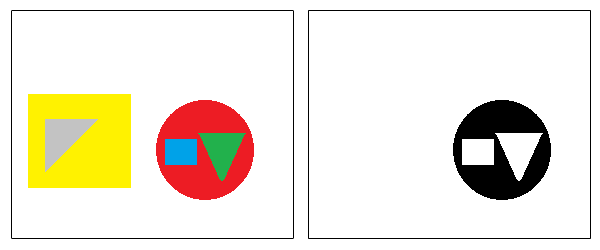
\includegraphics[scale=0.47]{graphics/threshold2.png}
		\caption{Ejemplo de filtrado threshold con umbral a 150}
		\label{fig:threshold2}
		\end{figure}
		
	Se trata de un algoritmo muy sencillo y rápido, pero en el que él éxito de los resultados depende tanto del umbral de entrada como de la imagen a analizar.
		
	\subsubsection{Adaptive Threshold}
	
	Se trata de una modificación del algoritmo anterior, donde el valor del umbral varía en cada región de la imagen. Este algoritmo también devuelve sólo una imagen binaria, pero aplica sobre ella un filtro más sofisticado que repara la mayor parte de los fallos del filtro anterior:

	\begin{center}
		$pixel(x,y) = \left\{
		\begin{array}{cc}
		MAXVAL 	& \text{ cuando } pixel(x,y) > T(x,y)\\ 
		0 	    & 	\text{e.o.c.}
		\end{array}\right.$
	\end{center}
	
	El umbral ya no es constante, sino que se convierte en el término $T(x,y)$ depende tanto de $x$ como de $y$. Existen muchas formas de calcular este término, pero en nuestro caso se calcula mediante la suma ponderada de los píxeles vecinos al $(x,y)$ dentro de un bloque de $3\times3$ píxeles donde el centro es el pixel a transformar. Tras haber realizado la suma, se le resta una constante teórica c, que especifica cuánto debe alejarse el valor de un píxel dado respecto al de la media calculada para que se considere que ha sobrepasado el umbral. En la implementación de este filtro se usará 3 como valor de esta constante, ya que proporciona resultados acordes a nuestros intereses.
	
	Con esta especificación, los resultados obtenidos son los mostrados en la Figura~\ref{fig:adaptive}. Como se puede observar, el resultado del filtro no depende de ningún valor y es más fiel que la mayoría de los resultados del threshold para figuras con este grado de simplicidad.\\
	
		\begin{figure}[!htbp]
		\centering
		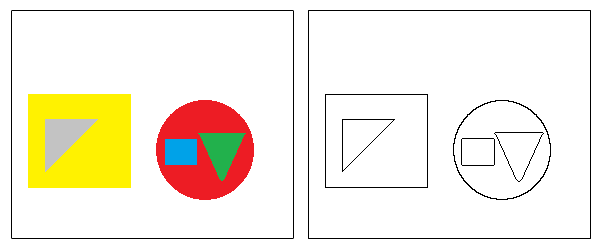
\includegraphics[scale=0.47]{graphics/adaptive.png}
		\caption{Ejemplo de filtrado adaptive threshold}
		\label{fig:adaptive}
		\end{figure}
	
	\subsubsection{Canny}
	
	Usando como base el algoritmo de detección de bordes creado por John F. Canny en 1986 (cuya especificación se puede ver en \cite{pajares}), este filtro aborda el problema de la detección de figuras de una forma diferente: en vez de detectar el contenido de la figura, detecta el perímetro de las mismas.\\
	
	Usando el algoritmo de canny, que también devuelve una única imagen, se obtiene el resultado mostrado en la Figura~\ref{fig:canny}.\\
	
		\begin{figure}[!htbp]
		\centering
		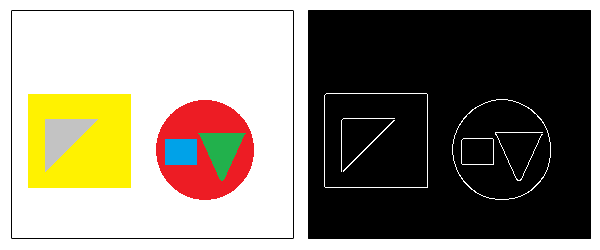
\includegraphics[scale=0.47]{graphics/canny.png}
		\caption{Ejemplo de filtrado canny}
		\label{fig:canny}
		\end{figure}
		
	Esta nueva aproximación produce resultados satisfactorios, pero origina nuevos problemas: el perímetro detectado en el algoritmo puede no estar cerrado, provocando que la figura resultante no se represente de forma correcta en la estructura de salida.
	
	\subsubsection{Hue Division}
	
	Este algoritmo se basa en un concepto más simple: buscar manchas de color como agrupaciones de píxeles vecinos con colores ``parecidos''. Es decir, se dividen los tres canales de color en diferentes rangos, y se agrupan los píxeles contiguos cuyos valores de color caigan dentro de un mismo rango en todos los canales.\\
	
	Para establecer los rangos, se divide cada canal de color (rojo, verde y azul) en un número $n$ de intervalos. El parámetro $n$ es de entrada y común para los tres canales. De esta forma, se recorre la imagen por cada intervalo existente de colores, devolviendo las figuras encontradas en cada intervalo en imágenes de salida distintas.\\
	
	Por ejemplo, si $n$ es 3, quiere decir que por cada canal se establecerán 3 intervalos, en total cada color podrá caer dentro de uno de los $3*3*3=27$ intervalos. Por cada intervalo se devuelve una imagen con las figuras presentes en él, comprobando antes que no esté vacía (no existen figuras con colores dentro de ese intervalo). Se puede ver un ejemplo en la Figura~\ref{fig:huedivision}.
	
		\begin{figure}[!htbp]
		\centering
		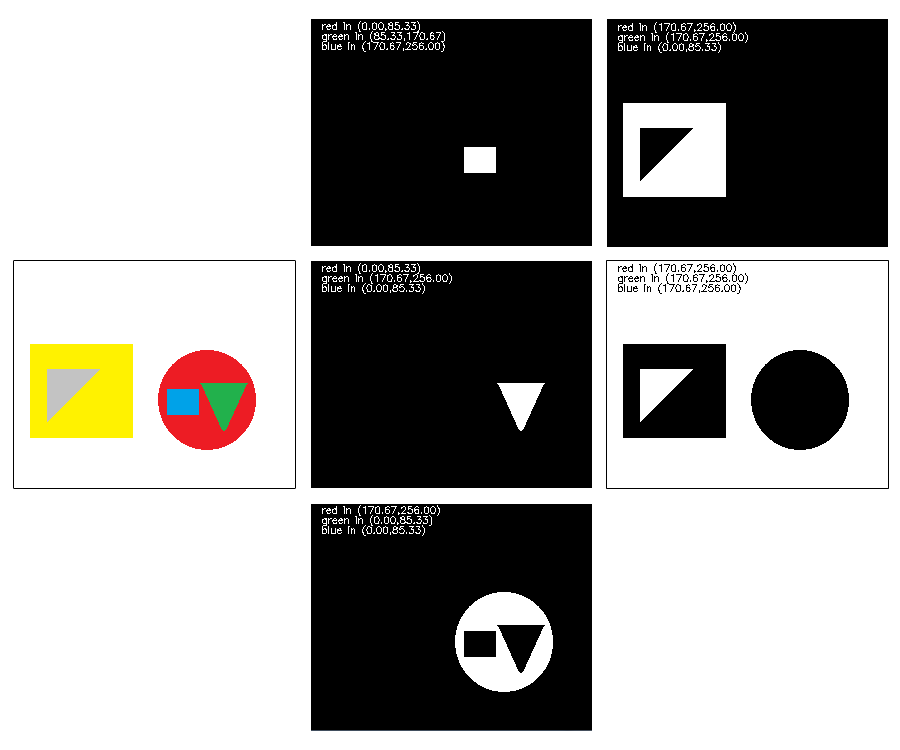
\includegraphics[scale=0.40]{graphics/huedivision.png}
		\caption{Ejemplo de filtrado hue division}
		\label{fig:huedivision}
		\end{figure}
	
	\subsubsection{Color Threshold}

	Se trata de una expansión del filtro Threshold para intentar resolver uno de sus principales problemas: dado que el filtro Threshold convierte la imagen en escala de grises para buscar píxeles que superen el umbral, puede darse el caso de que dos figuras con colores distintos se conviertan en el mismo tono de gris al convertirse a escala de grises. Este problema es independiente del método de transformación de RGB a escala de grises, e inherente al proceso en sí: al pasar de tres canales de color a un único canal, necesariamente varios valores de entrada van a coincidir en el mismo valor de salida (la función es sobreyectiva y el dominio de entrada es más grande que el de salida).\\
	
	Para resolver ese fallo, se realiza un filtro Threshold con tres umbrales distintos, uno para cada canal de color. Dado que estos umbrales van a poder ser manipulados por el usuario, se transformará previamente la imagen de RGB (rojo, verde y azul) a HSV (matiz, saturación y valor), que es un modelo más intuitivo para el ojo humano.\\
	
	Se pueden ver diferentes resultados de este filtro en las Figuras~\ref{fig:colorthres1} y ~\ref{fig:colorthres2}.
	
		\begin{figure}[!htbp]
		\centering
		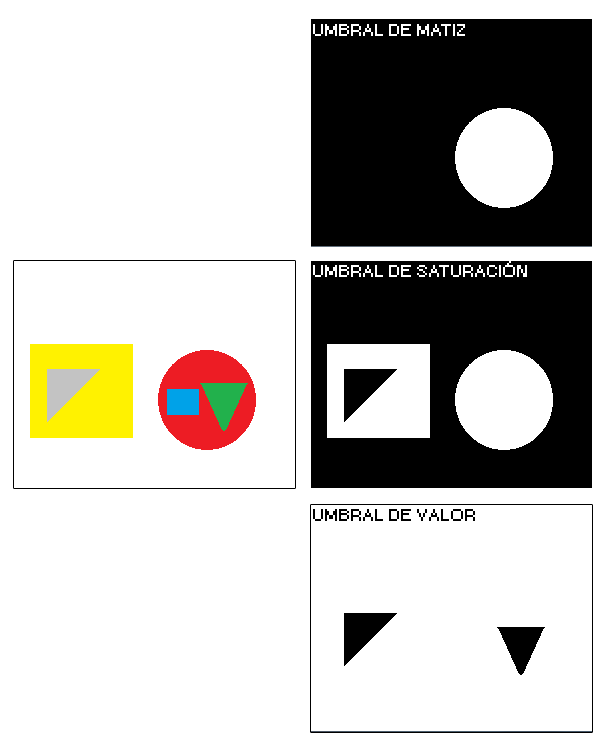
\includegraphics[scale=0.47]{graphics/colorthreshold.png}
		\caption{Ejemplo de filtrado color threshold: $Umbral_{H} = 55, Umbral_{S} = 150, Umbral_{V} = 205$}
		\label{fig:colorthres1}
		\end{figure}
	
		\begin{figure}[!htbp]
		\centering
		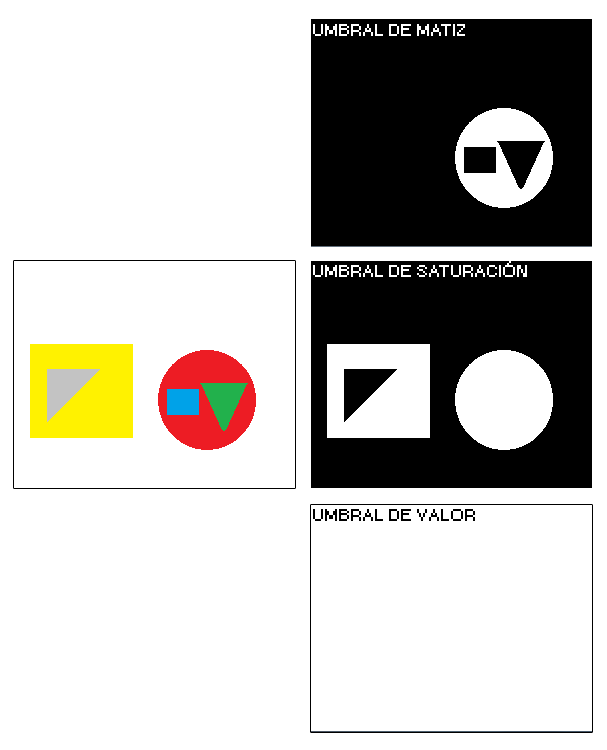
\includegraphics[scale=0.47]{graphics/colorthreshold2.png}
		\caption{Ejemplo de filtrado color threshold: $Umbral_{H} = 105, Umbral_{S} = 100, Umbral_{V} = 125$}
		\label{fig:colorthres2}
		\end{figure}
	
	
	
	\subsection{Detección de contornos y aproximación a polígonos}
	\label{sec:deteccionContornos}
	
	Una vez que tenemos la lista de imágenes binarias con las figuras localizadas, debemos proceder a representarlas en forma de polígonos. Para ello, primero detectaremos los contornos y posteriormente aproximaremos los mismos a polígonos.\\
	
	Para la primera parte (detección de contornos en base a una imagen binaria) haremos uso de la función \emph{cvFindContours} de OpenCV, cuyo resultado se puede ver en la Figura~\ref{fig:findcontours}.\\
	
		\begin{figure}[!htbp]
		\centering
		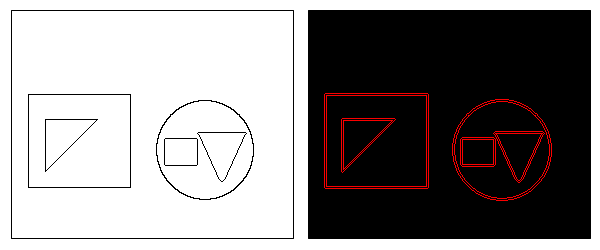
\includegraphics[scale=0.47]{graphics/contourdetection.png}
		\caption{Detección de contornos mediante OpenCV}
		\label{fig:findcontours}
		\end{figure}
		
	El ejemplo mostrado se ha basado en una imagen filtrada mediante el algoritmo Adaptive Threshold. Como se puede observar, una misma figura (el círculo) ha dado lugar a varios contornos. Este es un problema inherente a nuestro enfoque de detección de formas que se tratará más adelante.\\
	
	Posteriormente se usa otra función de OpenCV, \emph{cvApproxPoly}, para aproximar los contornos detectados a secuencias cerradas de vértices que podremos tratar con facilidad. El usuario puede decidir el grado de aproximación (de más simple a más fiel). Un ejemplo del resultado de esta función se ve en la Figura~\ref{fig:aproxpoly}\\
	
		\begin{figure}[!htbp]
		\centering
		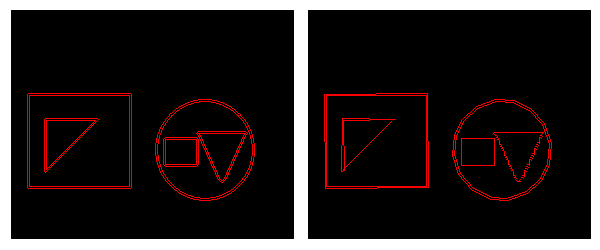
\includegraphics[scale=0.47]{graphics/aproxpoly.png}
		\caption{Aproximación de polígonos mediante OpenCV}
		\label{fig:aproxpoly}
		\end{figure}
				
	Teniendo los polígonos listados, sólo resta organizar la información obtenida y guardarla en un archivo XML.\\
	
	Para ello se procede a calcular el área de cada polígono. Si es menor que la especificada como ruido por el usuario (ver Guía de Usuario, Capítulo~\ref{chap:guiauso}), entonces se desechará. Si no, se almacenará dentro de la estructura de figuras a archivar en XML. El color de cada polígono, por otro lado, se calculará haciendo la media del color de todos los píxeles que contiene.\\
	
	Para acabar, necesitamos organizar los polígonos resultantes en estructura de árbol, de forma que los polígonos que se encuentran dentro de otro polígono sean sus hijos en el árbol resultante. Es aquí donde surge el principal problema del análisis de imágenes: \textbf{los polígonos repetidos}.\\
	
	Como ya hemos comentado anteriormente, una misma mancha de color puede originar varios contornos, debido a que la figura se ha detectado dos veces en el proceso de filtrado (por ejemplo, si se encuentra dentro de dos umbrales en el filtro Color threshold) o a que el proceso de detección de contornos ha devuelto dos contornos similares a la figura dada, por particularidades internas del algoritmo de OpenCV.\\
	
	Esto va a originar que, irremediablemente, haya ocasiones en las que aparecerán varios contornos (y posteriormente polígonos) similares. Se procede pues, antes de continuar el análisis, a eliminar los polígonos repetidos. Para ello, se comprueba primero que tengan el mismo número de vértices y que los rectángulos mínimos que los contienen tengan área y posición similares. Podría darse el caso de que un polígono A, teniendo más vértices que otro polígono B, se considerase idéntico a él, si se da uno de los dos siguientes casos: o bien un mismo vértice de B aproxima varios en A o bien en uno de los dos polígonos existe un ``vértice falso'' (es decir, el vértice intermedio de tres vértices alineados, que no aporta ninguna información nueva a la figura) en alguna arista. Sin embargo, la librería OpenCV nunca devuelve en un mismo polígono dos vértices lo suficientemente cercanos como para que sean considerados ``idénticos'' según nuestro criterio, por lo que no se estudiará ese caso. De la misma manera, la librería no genera nunca polígonos con ``falsos vértices'', por lo que se puede asegurar que dos polígonos no serán considerados idénticos (también serán denominados ``similares'') si tienen distinto número de vértices.\\

	Posteriormente, se procede a calcular si son efectivamente similares o no, es decir, si todos los vértices de un polígono tienen un vértice idéntico en el otro polígono y éstos pares siguen el ``orden'' de los polígonos (por ejemplo, si un vértice $v$ del polígono A es idéntico al vértice $v'$ del polígono B, entonces uno de los vértices contiguos a $v$ debe ser idéntico a uno de los vértices a $v'$ para que sean considerados idénticos). De una manera más formal:\\
		
	Sean dos polígonos A y B. Los polígonos serán similares, o considerados idénticos, si existe una disposición de vértices en A, $V_{A} = [v_{1}, v_{2}, ..., v_{n}]$, y otra en B, $V_{B} = [v'_{1}, v'_{2}, ..., v'_{n}]$ que asumen vértices contiguos tomados en sentido horario (o antihorario), tales que:
	
	\begin{center}
		$\forall k, 0 < k < N, dist(v_{k}, v'_{k}) < \epsilon$
	\end{center}
	
	Donde $N$ es el número de vértices de ambos polígonos que se deduce de la secuencia $v'_{1}, v'_{2}, ..., v'_{n}$ y $dist(p,q)$ es la función que calcula la distancia entre dos puntos del espacio bidimensional. La constante $\epsilon$ determina lo cerca que deben estar los vértices entre sí par considerarse idénticos.\\
	
		\begin{figure}[!htbp]
		\centering
		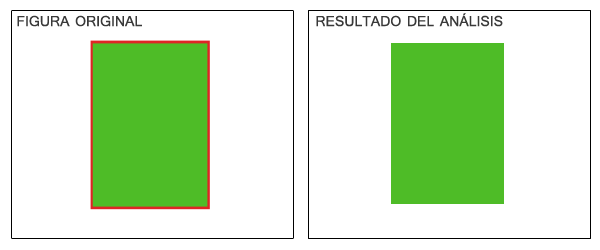
\includegraphics[scale=0.47]{graphics/reppoly.png}
		\caption{Caso de polígonos similares que no deben ser eliminados}
		\label{fig:colorsimilares}
		\end{figure}
	
	Sin embargo, puede darse el caso en que dos polígnos similares sean distintos y diferenciarse principalmente por el color (uno es la silueta del otro, ver Figura~\ref{fig:colorsimilares}. Dado que nunca trabajamos con el color, y éste se calcula \emph{a posteriori} (haciendo una media del color de los píxeles que contiene el polígono), no podremos usar el color de cada figura para distinguirlas, ya que sería bastante parecido (ambas figuras encierran aproximadamente los mismos píxeles), por lo que carecemos de la información necesaria debido a la naturaleza del proceso realizado. A pesar de todo, este caso es muy particular y no afecta al correcto desarrollo de la aplicación, por lo que no supone un problema en el análisis.\\
	
	Una vez eliminadas las figuras repetidas, se puede estructurar los polígonos en árboles, teniendo en cuenta que un polígono está dentro de otro cuando todos sus vértices están dentro de él. El rectángulo principal (que delimita el lienzo de la imagen) se elimina del análisis si ha sido detectado como polígono, ya que se encuentra en todas las imágenes y no aporta ninguna información relevante.\\
	
	El color calculado para cada polígono tenía en cuenta todos los píxeles que este contenía. Sin embargo, los polígonos que contienen otros polígonos han introducido información de más a la hora de calcular este color, ya que dentro de los polígonos que contienen se han tenido en cuenta los de sus hijos también. Es ahora que se conoce la estructura arbórea de la imagen cuando se pueden resolver estos detalles, recalculando el color de los polígonos que contienen a otros de forma que no se tenga en cuenta el color de sus polígonos internos.\\
	
	Una vez realizadas estas operaciones, los polígonos detectados en el análisis quedan tal y como se muestra en la Figura~\ref{fig:resfinal}.\\
	
		\begin{figure}[!htbp]
		\centering
		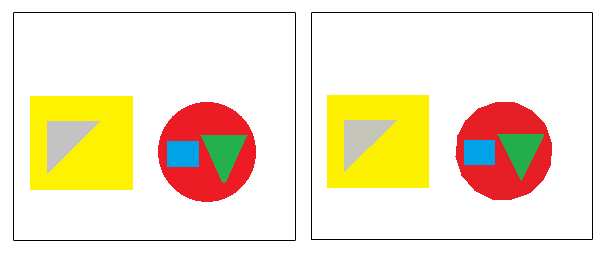
\includegraphics[scale=0.47]{graphics/anal_final_resul.png}
		\caption{Resultado final del análisis}
		\label{fig:resfinal}
		\end{figure}
	
	Finalmente, se guarda el contenido del análisis en un fichero XML, dando por terminado este proceso.
	
